\documentclass[paper=a4, fontsize=10pt]{scrartcl}
\usepackage[bottom=0.65in, left=0.5in, right=0.5in, top=0.65in, foot=0.4in]{geometry}
\usepackage{layouts}

\usepackage[usenames,dvipsnames,x11names]{xcolor}

\usepackage[T1]{fontenc}
\usepackage{fourier}
\usepackage[english]{babel}
\usepackage{amsmath,amsfonts,amsthm}

\usepackage{sectsty}
\allsectionsfont{\centering \normalfont\scshape}

\usepackage{acronym}
\usepackage{booktabs}
\usepackage{caption}
\usepackage{fancyhdr}
\usepackage{float}
\usepackage{graphicx}
\usepackage[htt]{hyphenat}
\usepackage{lastpage}
\usepackage{listings}
\usepackage{longtable}
\usepackage{minted}
\usepackage{multicol}

\usepackage{titlesec}

\usepackage[inline]{enumitem}

\usepackage{multirow}

\usepackage{tabularx}
\usepackage{ragged2e}
\newcolumntype{Y}{>{\RaggedRight\arraybackslash}X}

\usepackage{algorithm, algpseudocode}

\pagestyle{fancyplain}
\fancyhead{}
\fancyfoot[L]{}
\fancyfoot[C]{\thepage~of~2}
\renewcommand{\headrulewidth}{0pt}
\renewcommand{\footrulewidth}{0pt}
\setlength{\headheight}{13.6pt}

\newcommand{\horrule}[1]{\rule{\linewidth}{#1}}

\usepackage{tikz}
\usetikzlibrary{plotmarks}
\usepackage{pgfplots, pgfplotstable}
\pgfplotsset{compat=1.5}
\usepgfplotslibrary{colorbrewer}
\usepgfplotslibrary{fillbetween}
\usepgfplotslibrary{groupplots}

\titlespacing*{\section}
{0pt}{1.25ex plus .25ex minus .25ex}{1.25ex plus .25ex minus .25ex}

% http://tex.stackexchange.com/questions/67895/is-there-an-easy-way-of-using-line-thickness-as-error-indicator-in-a-plot

% Takes six arguments: data table name, x column, y column, error column,
% color and error bar opacity.
% ---
% Creates invisible plots for the upper and lower boundaries of the error,
% and names them. Then uses fill between to fill between the named upper and
% lower error boundaries. All these plots are forgotten so that they are not
% included in the legend. Finally, plots the y column above the error band.
\newcommand{\errorband}[6]{
\pgfplotstableread{#1}\datatable
  \addplot [name path=pluserror,draw=none,no markers,forget plot]
    table [x={#2},y expr=\thisrow{#3}+\thisrow{#4}] {\datatable};

  \addplot [name path=minuserror,draw=none,no markers,forget plot]
    table [x={#2},y expr=\thisrow{#3}-\thisrow{#4}] {\datatable};

  \addplot [forget plot,fill=#5,opacity=#6]
    fill between[on layer={},of=pluserror and minuserror];

  \addplot [#5,thick,no markers]
    table [x={#2},y={#3}] {\datatable};
}

\newacro{GA}{Genetic Algorithm}
\newacro{MDVRP}{Multi-Depot Vehicle Routing Problem}

\title{
\vspace{-1cm}
\normalfont \normalsize
\textsc{Norwegian University of Science and Technology\\IT3708 -- Bio-Inspired Artificial Intelligence}
\horrule{0.5pt} \\[0cm]
\Huge Project 2:\\ Solving the Multi-Depot Vehicle-Routing Problem\\using Genetic Algorithms\\[-0.3cm]
\horrule{2pt} \\[0.1cm]
}

\author{Per Magnus Veierland\\permve@stud.ntnu.no}

\date{\normalsize\today}

\begin{document}

\maketitle

\begin{multicols}{2}

\section*{Chromosome representation}

The chromosome is represented as a list of fixed length equal to the total number of depots ($t$). Each entry in the list consists of a list of variable length, with each entry representing a route assigned to the associated depot. Each of the routes is a variable length list consisting of the integer indexes of the customers visited on the route, depots not included. Flattening out this nested list structure will always yield a list with a length equal to the total number of customers $n$.

\section*{Creation}

Creating the initial chromosome population is done in a two-step process consisting of
\begin{enumerate*}[label=\alph*)]
    \item \textit{grouping} the set of customers such that each customer is assigned to its nearest depot,
    \item \textit{routing} and \textit{scheduling}, where for each depot customers are assigned and sequenced within routes.
\end{enumerate*}

Assuming that there are two depots $d_A$ and $d_B$, and a customer $c_i$ is to be assigned, the grouping works by assigning the customer to the closest depot as determined by the Euclidean distance.

If $\textsc{Distance}(c_i, d_A) < \textsc{Distance}(c_i, d_B)$, then assign $c_i$ to $d_A$. If $\textsc{Distance}(c_i, d_A) > \textsc{Distance}(c_i, d_B)$, then assign $c_i$ to $d_B$. Otherwise, if $\textsc{Distance}(c_i, d_A) = \textsc{Distance}(c_i, d_B)$, then assign $c_i$ to a depot randomly.

\begin{equation}
\textsc{Distance}(a, b) = \sqrt{(x_a - x_b)^2 + (y_a - y_b)^2}
\end{equation}

\vspace{0.2cm}

After grouping all customers to a depot, the \textit{Clarke and Wright Savings} algorithm~\cite{clarke1964scheduling} is used to assign customers to individual routes. The algorithm begins with assuming that a separate route is used for each customer, and that the cost of each route is $2 \cdot \textsc{Distance}(c_i, d)$. For each pair of customers $c_i, c_j$ assigned to a depot, the saving of combining their two routes is computed as $\textsc{Distance}(c_i, d) + \textsc{Distance}(c_j, d) - \textsc{Distance}(c_i, c_j)$, as the cost saved is one of the distances between the depot and each of the customers, and the added cost is the distance between the two customers.

After computing a list of the savings for combining each pair of customers within a depot, this list is sorted in descending order such that the list begins with the greatest saving. For each entry in the savings list, the following evaluation is made:

{
\begin{minipage}{\linewidth-4mm}
\begin{algorithm}[H]
\footnotesize
\begin{algorithmic}[1]
\Function{Best-Cost-Route-Crossover}{$p_1, p_2$}
    \State let $c_1 \gets \textsc{Copy}(p_1), c_2 \gets \textsc{Copy}(p_2)$
    \State let $\textit{depot\_index} \gets \textsc{RandomChoice}(V_d)$
    \State let $r_1 \gets \textsc{RandomChoice}(c_1[\textit{depot\_index}])$
    \State let $r_2 \gets \textsc{RandomChoice}(c_2[\textit{depot\_index}])$
    \For{$c$ \textbf{in} $r_1$}
        \State remove $c$ from each route in $c_2$
    \EndFor
    \State repeat lines 6-8 replacing $r_2$ for $r_1$ and $c_1$ for $c_2$
    \For{$c$ \textbf{in} $r_1$}
        \State let $\textit{insertion\_points} \gets []$
        \For{$\textit{depot\_routes}~\textbf{in}~c_2$}
            \For{$\textit{route}~\textbf{in}~\textit{depot\_routes}$}
                \State let $\textit{route\_cost} \gets \textsc{RouteCost}(\textit{route})$
                \For{$\textit{insert\_position}~\textbf{in}~\textsc{Range}(\textsc{Len}(\textit{route}) + 1)$}
                    \State let $\textit{modified} \gets \textsc{Copy}(\textit{route})$
                    \State \textbf{insert} $c$ at position \textit{insert\_position} into \textit{modified}
                    \State let $\textit{modified\_cost} \gets \textsc{RouteCost}(\textit{modified})$
                    \If{\textsc{WithinLimits}(\textit{modified})}
                        \State let $\textit{insertion\_cost} \gets \textit{modified\_cost} - \textit{route\_cost}$
                        \State \textbf{append} $(\textit{insertion\_cost}, \textit{route}, \textit{insert\_position})$
                    \EndIf
                \EndFor
            \EndFor
        \EndFor
        \State sort \textit{insertion\_points} in ascending order by \textit{insertion\_cost}
        \State let $(\textit{insertion\_cost}, \textit{route}, \textit{insert\_position}) \gets \textit{insertion\_points}[0]$
        \State \textbf{insert} $c_1$ at position \textit{insert\_position} into \textit{route}
    \EndFor
    \State repeat lines 10-29 replacing $r_2$ for $r_1$ and $c_1$ for $c_2$
    \State \textbf{return} $c_1, c_2$
\EndFunction
\end{algorithmic}
\caption{\textsc{Best Cost Route Crossover}}
\label{alg:bcrc}
\end{algorithm}
\end{minipage}
}

\begin{enumerate}[label=\alph*)]
    \item If $c_i$ and $c_j$ have neither been assigned a route and they can be added to a route within the duration and load constraints of their depot, a new route consisting of $c_i$ and $c_j$ is created.
    \item If exactly one of $c_i$ and $c_j$ has been assigned to a route, and it is adjacent to a depot within the route, the other customer is added into the route between the customer and the depot, if this modification does not violate the given duration and load constraints for their depot.
    \item If both $c_i$ and $c_j$ have been added to two different routes and are both adjacent to the depot in their routes, the two routes are merged into a single route with $c_i$ and $c_j$ in the middle, if the resulting route does not violate the duration and load constraints for their depot.
\end{enumerate}

Any remaining customers are assigned individual routes. The sequencing of the resulting routes are such that they work well as an input to the genetic algorithm, and no separate sequencing algorithm was found necessary.

\section*{Crossover operator}

\textit{Best-Cost-Route-Crossover} as developed in \cite{ombuki2006multi} was selected as the genetic operator for crossover to combine the chromosomes of individuals for inheritance, see Algorithm~\ref{alg:bcrc}. When applying it, a random route is selected from the same depot for both parents. The customers belonging to each of the selected routes are removed from the other parent. Further, the removed customers of each parent are reassigned to the feasible location with the lowest insertion cost. Insertion cost is given by the cost of a route after inserting a customer, minus the cost of a route before inserting a customer.

In 10\% of insertions, a random feasible insertion point is chosen instead of the best possible insertion point.

\section*{Mutation operator}

Inspired by the crossover operator, a \textit{Best-Cost-Customer-Mutation} genetic operator was developed to mutate individuals as a source of genetic diversity. In it, a random customer is selected and removed from the chromosome. In 90\% of cases, the customer is reinserted at the feasible location with the lowest insertion cost in the chromosome. In the other 10\% of cases, the customer is reinserted at a random feasible insertion point.

\section*{Selection mechanism}

The chosen parent selection mechanism is tournament selection, where to select a parent from the population a group of individuals are randomly chosen from the population. In $\epsilon$ of cases, a random individual is selected from the group as a parent, and in $1 - \epsilon$ of cases the individual in the group with the best fitness is selected as a parent.

\section*{Parameters}

Using a grid search, the best parameters was found to be a population size of 42, a tournament group size of 42, a tournament randomness factor $\epsilon$ of 0.1, a crossover rate of 0.42, and a mutation rate of 0.42.

\section*{Feasibility}

All individuals created are constructed as feasible solutions. The \textit{Best-Cost-Route-Crossover} genetic operator only produces feasible offspring as only route insertions are made which respect the duration and load constraints provided. The \textit{Best-Cost-Customer-Mutation} genetic operator only produces valid modifications, as any route insertion made must respect the duration and load constraints provided as well. In any case where the crossover or mutation operator fails to insert a customer to create a feasible route, the operators will return their input chromosomes.

\section*{Fitness function}

The primary objective of the assignment is to minimize the total distance travelled by all vehicles. To reflect this, the fitness of an individual $i$ is given by the sum of the distances of its routes $r \in \textit{routes}_i$. To simplify the notation it is assumed that both depot endpoints are contained in $r$, although this is not how the chromosome encodes it.

\begin{equation}
\textsc{Fitness}(i) = \sum_{r \in \textit{routes}_i}~\sum_{j=1}^{\vert{} r \vert{} - 1} \textsc{Distance}(r_j, r_{j+1})
\label{eq:fitness}
\end{equation}

As the genetic algorithm code is implemented to only support the maximizing of a fitness function, the reciprocal of Equation~\ref{eq:fitness} is used to transform maximizing into minimizing.

\section*{Elitism}

A low degree (0.01\%) of elitism is employed to ensure that the best solutions are not lost from the population during evolution. This is handled by sorting the population by fitness and always adding the elite individuals to the next generation before generating offspring to fill the rest of the next generation.

In addition to preserving the top solutions, elitism helps pressure the evolution process by sustaining the portion of top solutions within the population.

{
\vspace{0.3cm}
\centering
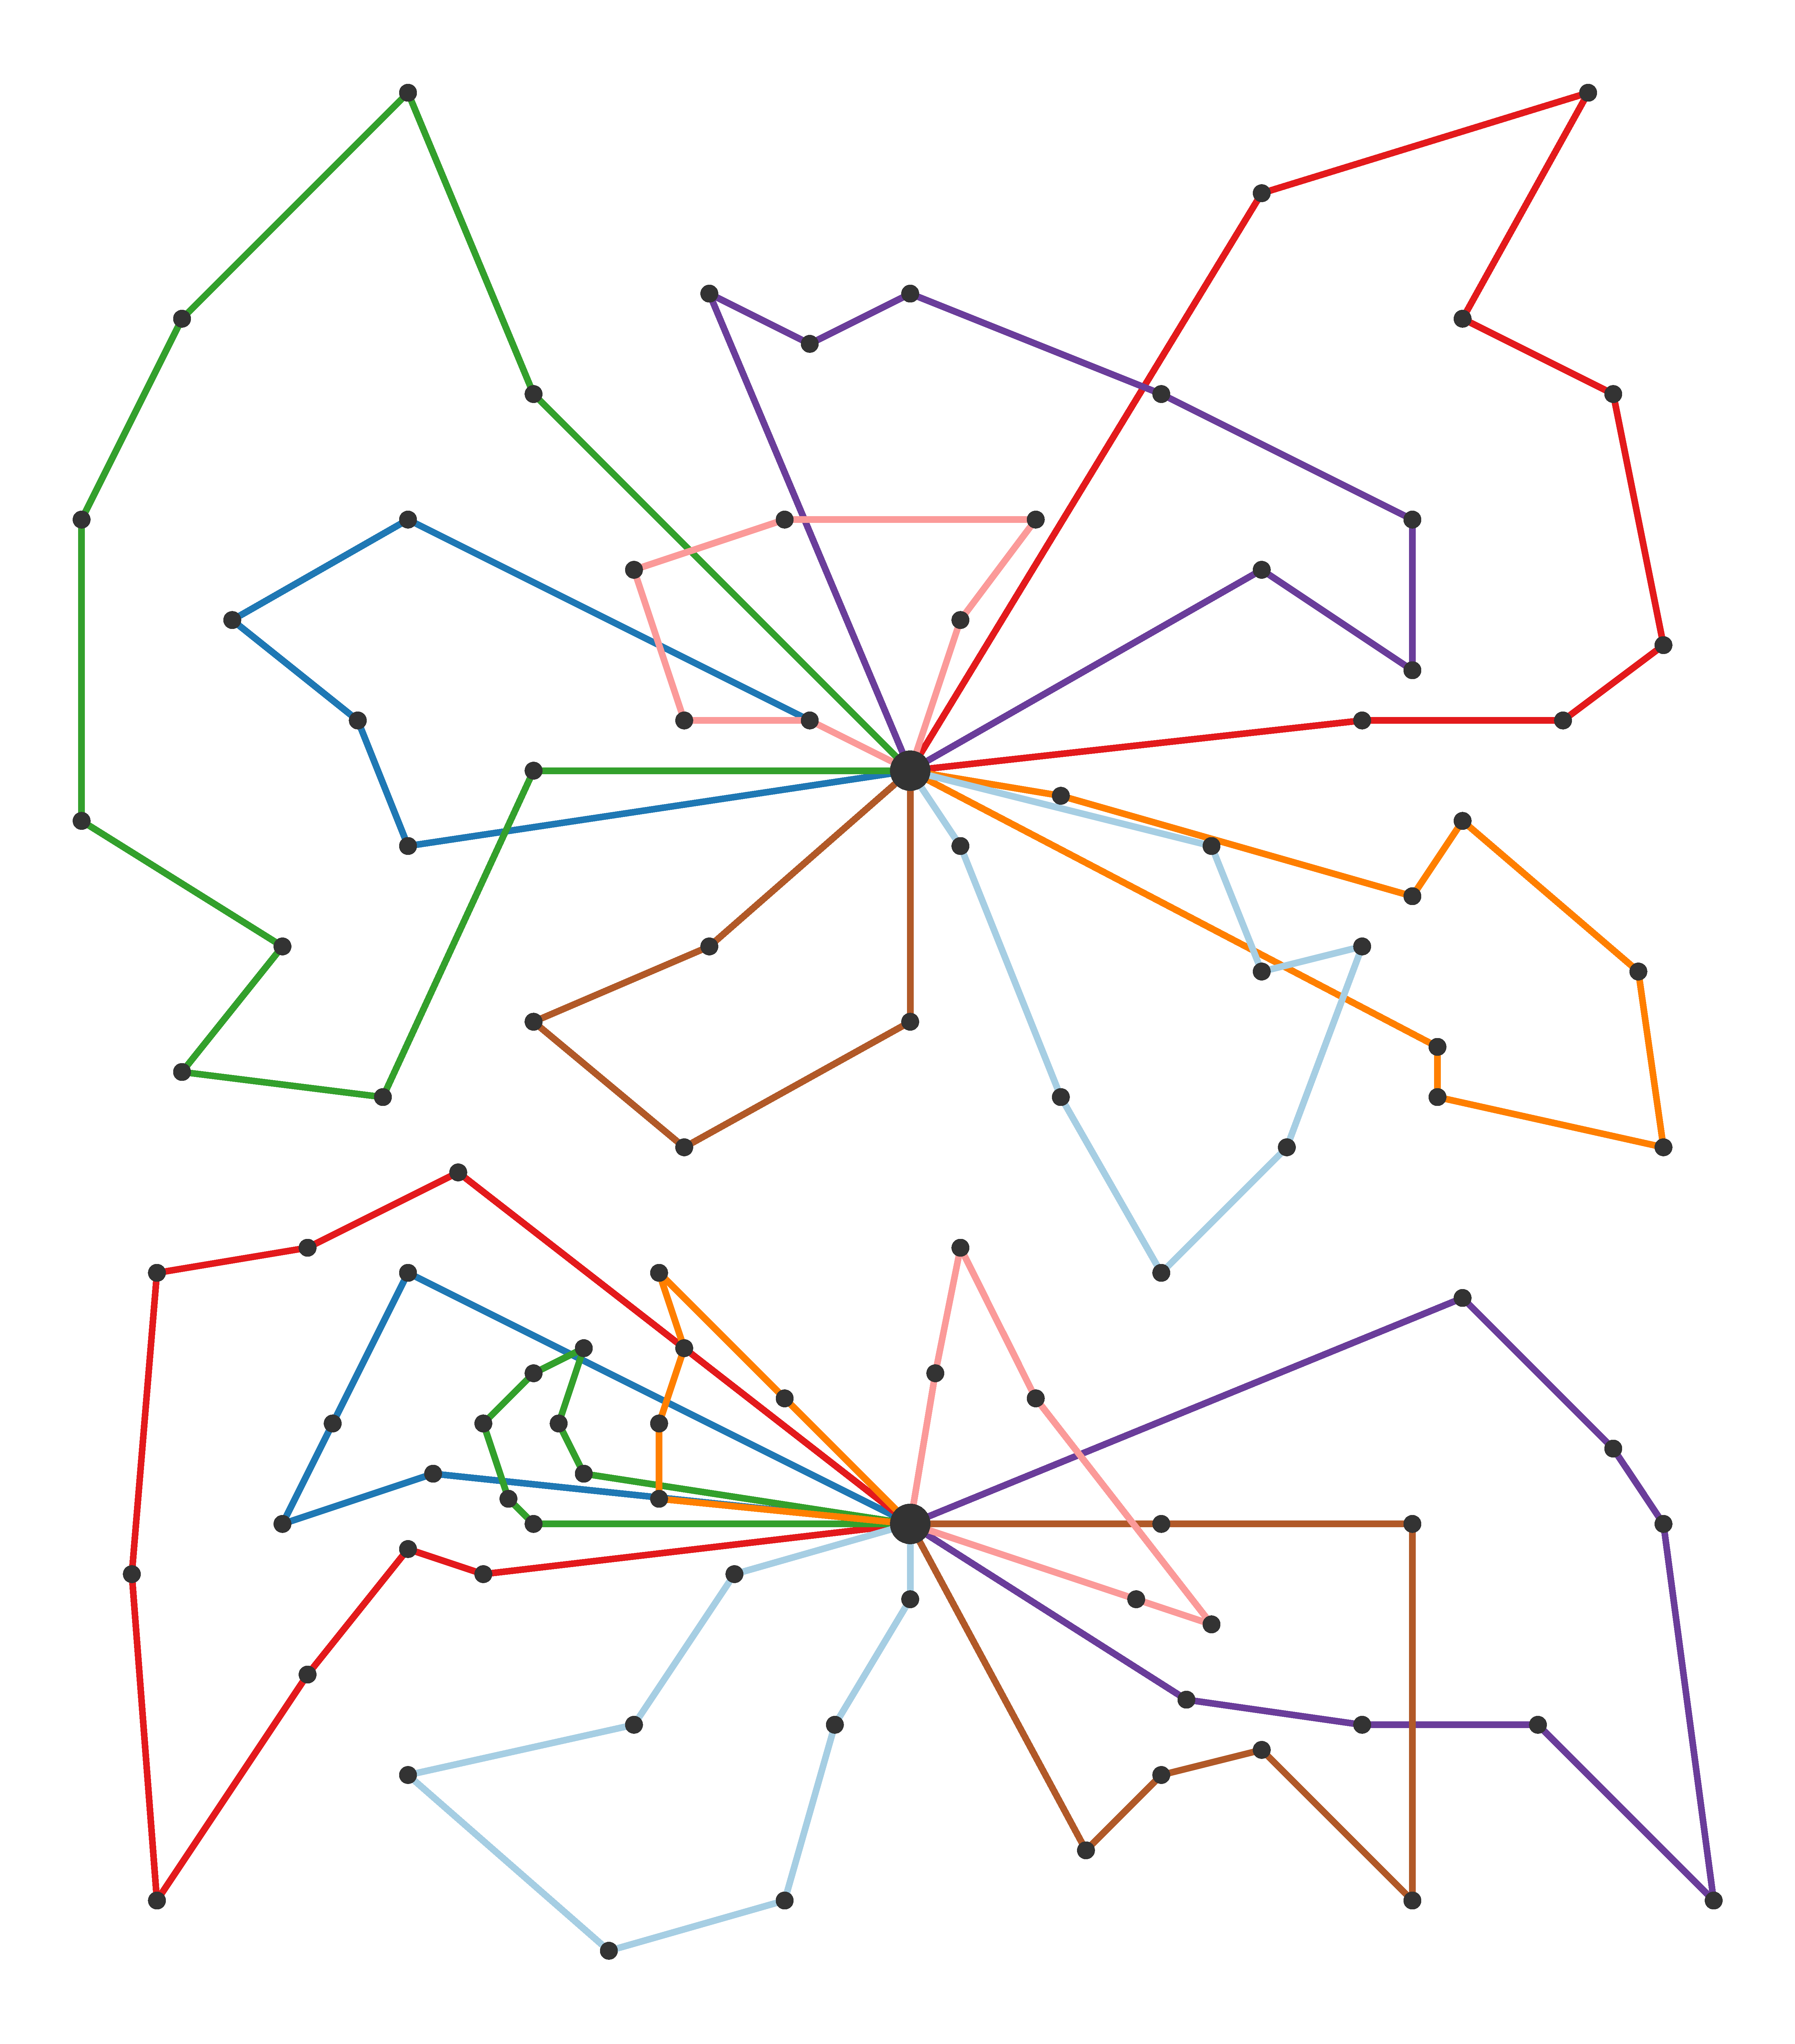
\includegraphics[scale=0.01]{figures/solution.pdf}
\captionof{figure}{Flatland visualization of baseline agent}
\label{figure:flatland_baseline}
\vspace{0.3cm}
}

{
\footnotesize
\begin{minted}[mathescape,
               numbersep=5pt,
               frame=lines,
               framesep=2mm,
               xleftmargin=3mm,
               xrightmargin=3mm]{text}
600.68
1   1   60.06   71   0 17 37 15 33 45 44 0
1   2   26.96   50   0 18 4 0
1   3   66.55   79   0 42 19 40 41 13 0
2   1   96.01   80   0 23 24 43 7 26 48 0
2   2   58.23   76   0 11 32 1 8 27 0
2   3   51.19   64   0 6 14 25 0
2   4   24.74   59   0 46 12 47 0
3   1   53.43   74   0 10 39 30 34 50 0
3   2   38.97   80   0 49 5 38 16 9 0
4   1   79.44   72   0 22 31 28 3 36 35 0
4   2   45.10   72   0 21 29 2 20 0
\end{minted}
\vspace*{-3mm}
\captionof{figure}{Solution to problem \texttt{p01}.}
\label{fig:code_delta_reinforcement}
}

\bibliographystyle{unsrt}
\bibliography{references.bib}

\end{multicols}

\end{document}
